\documentclass[a4paper, 12pt]{report}
\usepackage[T2A]{fontenc} 
\usepackage[utf8]{inputenc}
\usepackage[english,russian]{babel} 
\usepackage{amsmath,amsfonts,amssymb,amsthm,mathtools}
\usepackage[left=2cm,right=2cm,top=2cm,bottom=2cm,bindingoffset=0cm]{geometry}
\usepackage{graphicx}
\usepackage[linesnumbered,boxed]{algorithm2e}
\usepackage{verbatim}

\newenvironment{Proof} 
{\par\noindent{$\blacklozenge$}}
{\hfill$\scriptstyle\boxtimes$} 

\newenvironment{example} 
{\par\noindent{\textsc{\textbf{Пример}.}}} 
{\hfill$\scriptstyle\Box$} 

\newtheorem*{theorem}{Теорема} 
\newtheorem*{corollary}{Следствие}
\newtheorem*{lemma}{Лемма}

\newcommand{\RNumb}[1]{\uppercase\expandafter{\romannumeral #1\relax}}
\newcommand{\Rm}{\mathbb{R}}
\newcommand{\Cm}{\mathbb{C}}
\newcommand{\I}{\mathbb{I}}
\newcommand{\N}{\mathbb{N}}
\newcommand{\Z}{\mathbb{Z}}
\newcommand{\Q}{\mathbb{Q}}

\title{\textbf{\Huge{Методы вычислений}}\\Лабораторная работа 5\\«Итерационные методы решения проблемы собственных значений\\Выполнила Николаева Ксения, 9 группа}
\date{} 

\begin{document}
    \maketitle

    \textbf{\Huge{Постановка задачи}}\\\\
1. Реализовать метод скалярных произведений для нахождения наибольшего по модулю собственного значения симметричной матрицы.  \\
2. Реализовать итерационный метод вращений Якоби для нахождения всех собственных значений симметричной матрицы.  \\
3. Выполнить вычислительный эксперимент:  
   \begin{itemize}
       \item Сгенерировать случайную симметричную матрицу порядка $n = 10$.
       \item Использовать начальные данные для метода скалярных произведений ($\epsilon = 10^{-7}$, случайный начальный вектор).
       \item Для метода вращений Якоби использовать тот же критерий остановки ($\epsilon = 10^{-7}$).
   \end{itemize}
\newpage
\textbf{\Huge{Краткие теоретические сведения}}\\\\
\textbf{Метод скалярных произведений}
Метод скалярных произведений используется для нахождения наибольшего по модулю собственного значения симметричной матрицы.  

\textbf{Алгоритм метода:}  
\begin{enumerate}
    \item Задается начальный ненулевой вектор $y^{(0)}$ и нормализуется с использованием евклидовой нормы:
    \[
    u^{(0)} = \frac{y^{(0)}}{\|y^{(0)}\|_2}.
    \]
    \item На каждой итерации вычисляются:
    \[
    y^{(k+1)} = A \cdot u^{(k)},
    \]
    где $A$ — заданная матрица.
    \item Собственное значение на текущем шаге:
    \[
    \lambda^{(k+1)} = \langle y^{(k+1)}, u^{(k)} \rangle,
    \]
    где $\langle \cdot, \cdot \rangle$ — скалярное произведение.
    \item Нормализация вектора:
    \[
    u^{(k+1)} = \frac{y^{(k+1)}}{\|y^{(k+1)}\|_2}.
    \]
    \item Критерий сходимости:
    \[
    \|A u^{(k+1)} - \lambda^{(k+1)} u^{(k+1)}\|_2 < \epsilon.
    \]
\end{enumerate}

\textbf{Итерационный метод вращений Якоби}
Метод вращений Якоби используется для нахождения всех собственных значений симметричной матрицы.

\textbf{Алгоритм метода:}  
\begin{enumerate}
    \item Задается начальная матрица $A^{(0)}$.
    \item На каждой итерации выбирается элемент $a_{pq}$, который имеет максимальное значение среди внедиагональных элементов.
    \item Вычисляется угол поворота:
    \[
    \phi = \frac{1}{2} \arctan\left(\frac{2a_{pq}}{a_{pp} - a_{qq}}\right).
    \]
    \item Вычисляются коэффициенты вращения:
    \[
    c = \cos(\phi), \quad s = \sin(\phi).
    \]
    \item Матрица преобразуется согласно формулам:
    \[
    a_{pp}^{(k+1)} = c^2 a_{pp} + 2cs a_{pq} + s^2 a_{qq},
    \]
    \[
    a_{qq}^{(k+1)} = s^2 a_{pp} - 2cs a_{pq} + c^2 a_{qq},
    \]
    \[
    a_{pq}^{(k+1)} = 0, \quad a_{ij}^{(k+1)} = a_{ij} \text{ (для остальных элементов)}.
    \]
    \item Критерий сходимости:
    \[
    \sum_{i \neq j} (a_{ij}^{(k)})^2 < \epsilon.
    \]
\end{enumerate}

   \newpage
   \textbf{\Huge{Листинг программы с комментариями}}\\\\
   \begin{verbatim}
#include <bits/stdc++.h>

using namespace std;

// Генерация случайной симметричной матрицы
vector<vector<double>> generateSymmetricMatrix(int n) {
    vector<vector<double>> A(n, vector<double>(n, 0));
    srand(time(0));

    for (int i = 0; i < n; ++i) {
        for (int j = 0; j <= i; ++j) {
            A[i][j] = rand() % 201 - 100; // [-100, 100]
            A[j][i] = A[i][j];
        }
    }
    return A;
}

// Вычисление евклидовой нормы вектора
double euclideanNorm(const vector<double>& v) {
    double sum = 0;
    for (double x : v) {
        sum += x * x;
    }
    return sqrt(sum);
}

// Умножение матрицы на вектор
vector<double> multiplyMatrixVector(const vector<vector<double>>& A, const vector<double>& v) {
    int n = A.size();
    vector<double> result(n, 0);

    for (int i = 0; i < n; ++i) {
        for (int j = 0; j < n; ++j) {
            result[i] += A[i][j] * v[j];
        }
    }
    return result;
}

// Метод скалярных произведений
void powerIteration(const vector<vector<double>>& A, vector<double> y0, double epsilon) {
    int n = A.size();
    vector<double> u_k = y0;
    double norm = euclideanNorm(u_k);

    // Нормировка начального вектора
    for (double& x : u_k) {
        x /= norm;
    }

    int iteration = 0;
    double lambda1 = 0;
    vector<double> residual;

    while (true) {
        ++iteration;

        // Вычисление y^(k+1)
        vector<double> y_k1 = multiplyMatrixVector(A, u_k);

        // Вычисление lambda_1^(k+1)
        lambda1 = 0;
        for (int i = 0; i < n; ++i) {
            lambda1 += y_k1[i] * u_k[i];
        }

        // Нормировка: u^(k+1) = y^(k+1) / ||y^(k+1)||
        double norm_yk1 = euclideanNorm(y_k1);
        for (int i = 0; i < n; ++i) {
            u_k[i] = y_k1[i] / norm_yk1;
        }

        // Вычисление невязки: ||A * u^(k) - lambda1 * u^(k)||
        vector<double> Au_k = multiplyMatrixVector(A, u_k);
        residual.resize(n);
        for (int i = 0; i < n; ++i) {
            residual[i] = Au_k[i] - lambda1 * u_k[i];
        }
        double residualNorm = euclideanNorm(residual);

        if (residualNorm < epsilon) {
            cout << "Точность достигнута на итерации: " << iteration << endl;
            cout << "Приближенное наибольшее по модулю собственное значение: " << lambda1 << endl;
            cout << "Вектор невязки: \n[";
            for (double x : residual) {
                cout << x << "\n";
            }
            cout << "]\n";
            cout << "||A * u^(k) - lambda1 * u^(k)||2: " << residualNorm << endl;
            return;
        }

        if (iteration > 1000) {
            cout << "Итерационный процесс расходится." << endl;
            return;
        }
    }
}


// Сумма квадратов внедиагональных элементов
double sumOffDiagonal(const vector<vector<double>>& A) {
    int n = A.size();
    double sum = 0;
    for (int i = 0; i < n; ++i) {
        for (int j = 0; j < n; ++j) {
            if (i != j) {
                sum += A[i][j] * A[i][j];
            }
        }
    }
    return sum;
}

// Метод вращений Якоби
void jacobiRotationMethod(vector<vector<double>> A, double epsilon) {
    int n = A.size();
    int iterations = 0;

    while (sumOffDiagonal(A) >= epsilon) {
        ++iterations;

        // Поиск наибольшего внедиагонального элемента
        int p = 0, q = 0;
        double maxElem = 0;
        for (int i = 0; i < n; ++i) {
            for (int j = i + 1; j < n; ++j) {
                if (fabs(A[i][j]) > fabs(maxElem)) {
                    maxElem = A[i][j];
                    p = i;
                    q = j;
                }
            }
        }

        // Вычисление угла поворота
        double phi = 0.5 * atan2(2 * A[p][q], A[p][p] - A[q][q]);
        double c = cos(phi);
        double s = sin(phi);

        // Преобразование матрицы
        vector<vector<double>> A_next = A;
        for (int i = 0; i < n; ++i) {
            if (i != p && i != q) {
                A_next[i][p] = c * A[i][p] + s * A[i][q];
                A_next[p][i] = A_next[i][p];
                A_next[i][q] = -s * A[i][p] + c * A[i][q];
                A_next[q][i] = A_next[i][q];
            }
        }
        A_next[p][p] = c * c * A[p][p] + 2 * c * s * A[p][q] + s * s * A[q][q];
        A_next[q][q] = s * s * A[p][p] - 2 * c * s * A[p][q] + c * c * A[q][q];
        A_next[p][q] = 0;
        A_next[q][p] = 0;

        A = A_next;
    }

    // Вывод результатов
    cout << "Итерации: " << iterations << endl;
    cout << "Собственные значения:" << endl;
    for (int i = 0; i < n; ++i) {
        cout << A[i][i] << "\n";
    }
    cout << endl;
    cout << "Сумма квадратов внедиагональных элементов: " << sumOffDiagonal(A) << endl;
}

int main() {

    setlocale(LC_ALL, "Russian");
    freopen ("output.txt", "w", stdout);

    int n = 10;
    double epsilon = 1e-7;

    // Генерация симметричной матрицы
    vector<vector<double>> A = generateSymmetricMatrix(n);

    // Вывод матрицы
    cout << "Матрица A:" << endl;
    for (const auto& row : A) {
        for (double x : row) {
            cout << x << " ";
        }
        cout << endl;
    }

    // Начальный вектор y^(0)
    vector<double> y0(n, 1.0);

    // Вывод начального вектора
    cout << "Начальный вектор y^(0): [";
    for (double x : y0) {
        cout << x << " ";
    }
    cout << "]\n";

    // Запуск метода
    powerIteration(A, y0, epsilon);

    cout << "\n-----------------------------------\n";

    // Запуск метода Якоби
    jacobiRotationMethod(A, epsilon);

    return 0;
}

   \end{verbatim}
   \newpage
   \textbf{\Huge{Результаты}}\\\\

   \begin{center}
        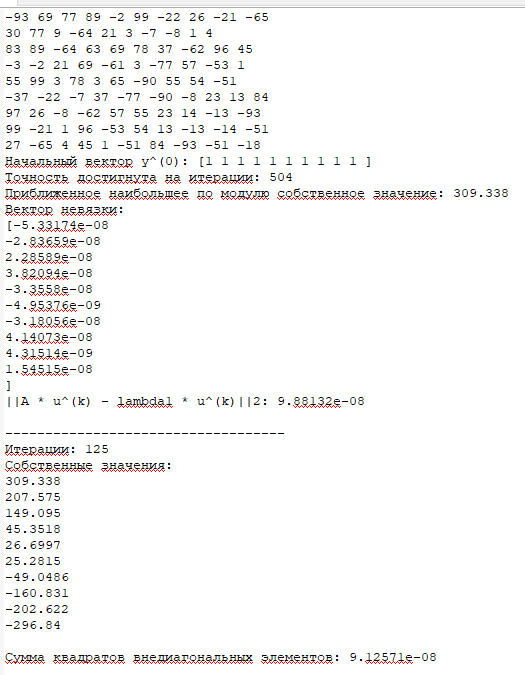
\includegraphics[scale = 0.99]{pic13.png}
   \end{center}

   

    \newpage
   \textbf{\Huge{Выводы}}\\\\
   $\bullet$ Метод скалярных произведений эффективно находит наибольшее по модулю собственное значение, однако не подходит для нахождения остальных значений.\\
   $\bullet$ Метод вращений Якоби позволяет найти все собственные значения, но требует большего числа итераций и вычислений.\\
   $\bullet$ Проведенные эксперименты подтвердили правильность реализации алгоритмов и их сходимость при заданной точности $\epsilon = 10^{-7}$.\\
    $\bullet$ Оба метода работают корректно для симметричных матриц, что соответствует теоретическим ожиданиям.\\

   
\end{document}


